\documentclass{article}
\usepackage[T1]{fontenc}
\usepackage{lmodern}
\usepackage{graphicx}
\usepackage{amsmath,amssymb}
\usepackage[a4paper,margin=2cm]{geometry}
\usepackage[absolute,overlay]{textpos}
\setlength{\TPHorizModule}{1mm}
\setlength{\TPVertModule}{1mm}
\usepackage[indonesian]{babel}
\usepackage{hyperref}
\setlength{\emergencystretch}{2em}
% unit: Halaman 18

\begin{document}

% === Halaman 18 (llm) ===

\vspace{127.71mm}

(a) Citra orisinal \vspace{10mm} (b) Citra hasil enhanced LSB \vspace{10mm} (c) Citra stego \vspace{10mm} (b) Citra hasil enhanced LSB

\vspace{100.98mm}

% deskripsi: Ilustrasi proses steganografi: Gambar (a) menampilkan citra orisinal Doraemon, panah biru mengarah ke gambar (b) yang menunjukkan hasil ekstraksi bit LSB (enhanced LSB) yang terlihat seperti noise berwarna.
% bbox normalisasi: [0.2480, 0.0900, 0.7050, 0.5200]
\begin{textblock*}{95.97mm}(52.08mm,26.73mm)
\noindent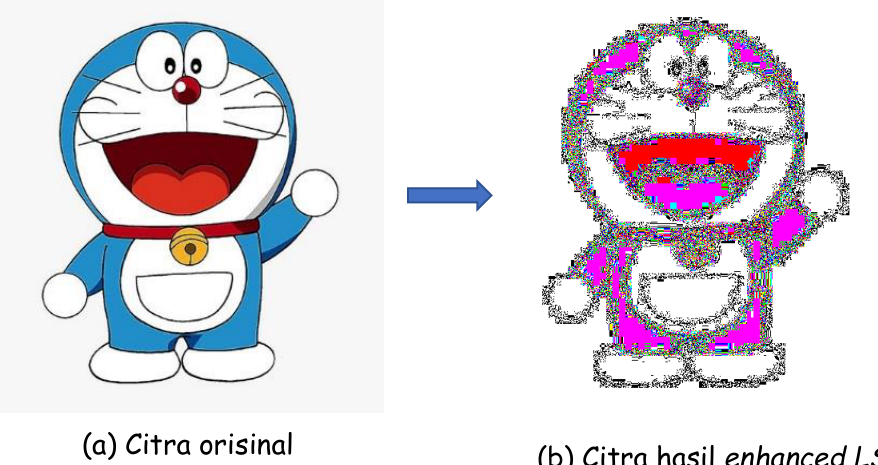
\includegraphics[width=95.97mm,height=127.71mm]{../../images/llm/page_018_img_01.png}%
\end{textblock*}

% deskripsi: Ilustrasi proses steganografi: Gambar (c) menampilkan citra stego (citra yang sudah disisipi pesan), panah biru mengarah ke gambar (b) di bawahnya yang menunjukkan hasil ekstraksi bit LSB (enhanced LSB).
% bbox normalisasi: [0.2780, 0.5500, 0.7220, 0.8900]
\begin{textblock*}{93.24mm}(58.38mm,163.35mm)
\noindent
\includegraphics[width=93.24mm,height=100.98mm]{../../images/llm/page_018_img_02.png}%
\end{textblock*}

\end{document}
